\documentclass[titlepage]{article}
\usepackage[tc]{titlepic}
\usepackage{graphicx}
\usepackage{amsmath}
\usepackage[top=25mm, bottom=25mm, left=27mm, right=27mm]{geometry}
\usepackage{caption}
\usepackage{listings}
\usepackage{lstlangarm}
\usepackage{tabu}
\usepackage[outdir=./]{epstopdf}


\date{}
\author{Erdal Sidal Dogan\\ \#041702023  \and Alp
	Gokcek \\ \#041701014}
\title{
\includegraphics[width=0.6\textwidth]{../images/logo_en_color.png}\\ 
\vspace{5em}
EE306 - Microprocessors\\
\vspace{2em}
\textbf{Lab 1 \linebreak Using Logic Instructions with the ARM Processor
}\\
\vspace{1.5em}
February 17, 2020}

\begin{document}
	\maketitle
	\section{Longest Alternating Strings}
	Our approach for this problem was to utilize the \emph{XOR} operation. We XORed the input string with another string that consist of alternating 1's and 0's. Given that XOR of two different bits always results in 1, when we XOR the input  with the alternating string, longest sequence of 1's in the output should give the longest sequence of alternating bits in the input also. The problem is that we didn't knew wheter the first bit of longest alternating string was 1 or 0.  This was a problem because the answer was either the length of longest sequence of 0's or 1's inthe output string, depending on the first bit of alternating sequence in input string.  \\
	
	\begin{minipage}{0.5\textwidth}
		\begin{equation*}
			\begin{tabular}{r@{\;}r}
				& 101101010001  \\
				\tiny{XOR} & 101010101010\\
				\hline
				& 000111111011
			\end{tabular}
		\end{equation*}
	\end{minipage}
	\quad
	\begin{minipage}{0.35\textwidth}
		\begin{equation*}
				\begin{tabular}{r@{\;}r}
				& 101101010001  \\
				\tiny{XOR} & 010101010101\\
				\hline
				& 111000000100
			\end{tabular}
		\end{equation*}
	\end{minipage}
	\\

	Above you can see the input string 101101010001 is being XORed with two alternating strings, one of them starts with 1 and other with 0. Using two alternating strings is to address the problem mentioned in previous paragraph, unknown start bits of the longest alternating string. What we did in order to solve this problem is, we used XOR operation for two different alternating strings. We know that the lenght of the longest sequence of 1's in the result of XOR operation is equal to the lenght of longest alternating bits in the input. We count length of longest sequence of 1's in both XOR outputs, the greater number is our answer.\\
	
	\lstinputlisting[language={[ARM]Assembler}, frame=single, basicstyle=\ttfamily, caption=Assembly Code for finding longest string of alternating 1's and 0's]{../source_codes/task-iii.s}
	
		\begin{figure}[th]
		\centering
		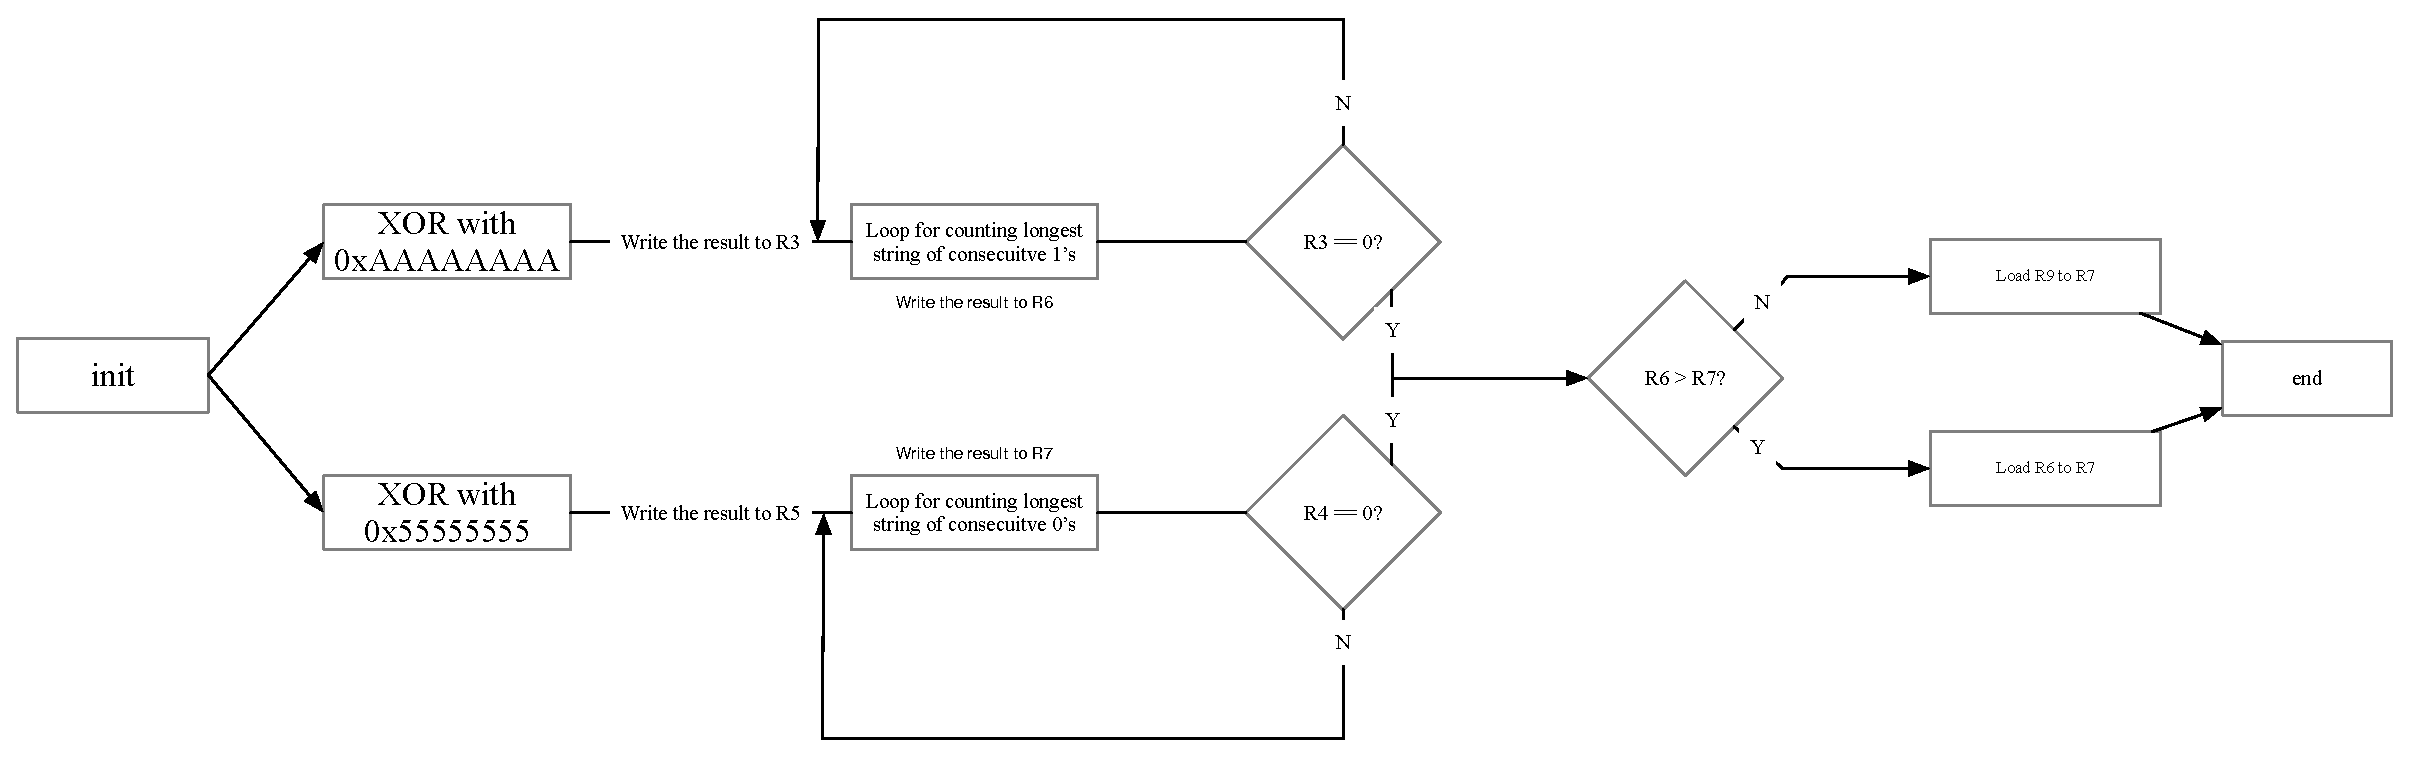
\includegraphics[scale=.4]{../images/task-iii.eps}
		\caption{Longest Sequnce of Alternating 1's and 0's Flowchart}
	\end{figure}

	\section{Parity Bit}
	Our approach for this problem was to sum all the bits in the binary number and check whether it is odd or even. In the first part, we have calculated the bitwise sum of all bits in the given number. We have taken the bitwise \emph{AND} operation of the input string with hexadecimal number 0x1 and stored the result in a register. Given that AND operation of 1 with another bit always results in the other bits value, when we AND the input with the 1, we get the value of LSB (least significant bit). Then we shifted the input string to the right by 1 bit which cleared the LSB. In the final part of the calculating bitwise sum of all bits in the input string, we add the result of \emph{AND} operation that stored in a register with the current value of the sum of bits. This process continues until the input string is equal to hexadecimal number 0x0. In the last part, we checked whether the sum of all bits LSB is 1 or 0. If it is 1 then the sum is odd which makes the even parity bit 1 and odd parity bit 0. If it is 0 then the sum is even which makes the even parity bit 0 and the odd parity bit 1. After checking last bit we did clear the MSB (most significant bit) and LSB and calculated the logical \emph{OR} operation with hexadecimal number 0x80000000 if the even parity bit is 1, else we ORed with hexadecimal number 0x00000001. 
	\lstinputlisting[language={[ARM]Assembler}, frame=single, basicstyle=\ttfamily, caption= Assembly code for finding the odd and even parity bits]{../source_codes/task-iv.s}
	
	\begin{figure}[th]
		\centering
		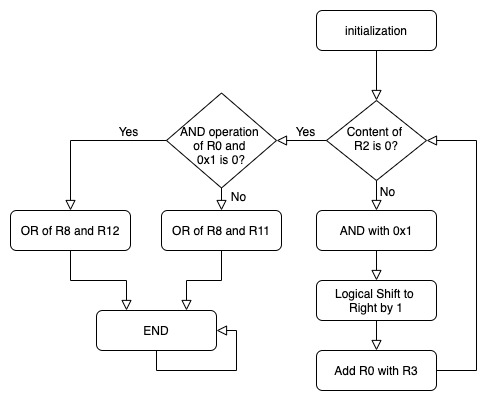
\includegraphics[scale=.6]{../images/flowchart_2.jpg}
		\caption{Parity Bit detection flowchart}
	\end{figure}

\end{document}